\section{Beyond Physical Memory: Mechanisms}

%------------------------------------------------
\begin{frame}{Relaxing a Big Assumption}

\begin{itemize}
    \item So far: every address space of every running process
          \textbf{fits into physical memory}.
    \item Now: support \textbf{many concurrently-running, large}
          address spaces.
    \item Requires an additional level in the \textbf{memory hierarchy}:
    \begin{itemize}
        \item more capacity than memory, and therefore slower;
        \item usually a \textbf{hard disk drive} (or a Flash-based SSD).
    \end{itemize}
\end{itemize}

\begin{block}{Crux: How to Go Beyond Physical Memory}
How can the OS make use of a larger, slower device to transparently
provide the illusion of a large virtual address space?
\end{block}

\end{frame}

%------------------------------------------------
\begin{frame}{Why a Single Large Address Space?}

\begin{itemize}
    \item \textbf{Convenience and ease of use}: write the program naturally,
          allocating memory as needed.
    \item Contrast with older systems that used \textbf{memory overlays}:
          programmers manually moved code or data in and out of memory.
    \item \textbf{Multiprogramming} almost demanded the ability to swap out
          pages: early machines could not hold all pages of all processes.
    \item Multiprogramming + ease of use $\Rightarrow$ use
          \textbf{more memory than is physically available}.
\end{itemize}

\end{frame}

%------------------------------------------------
\begin{frame}{Swap Space}

\begin{itemize}
    \item Space reserved on disk for moving pages back and forth
          (\textbf{swap out} / \textbf{swap in}), in page-sized units.
    \item The OS must remember the \textbf{disk address} of each swapped page.
    \item Its size determines the maximum number of pages in use at a time.
\end{itemize}

\begin{figure}
    \centering
    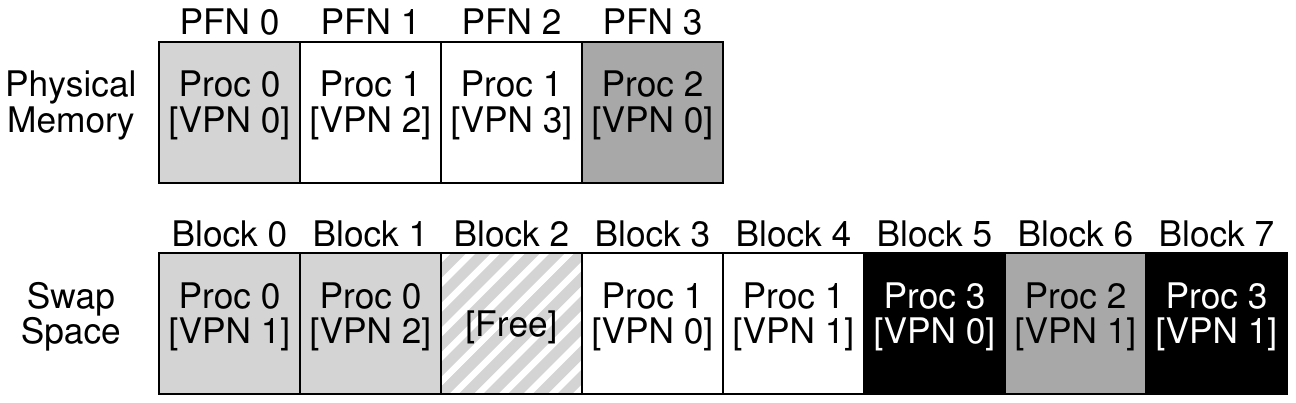
\includegraphics[width=0.70\linewidth]{figs/chapter-21/figure-21.1.png}
    \caption*{Source: chapter page 3.}
    \label{fig:figure-21.1}
\end{figure}

{\small
\begin{itemize}
    \item 4-page physical memory, 8-page swap space; Proc 3 is entirely
          swapped out. Code pages of a binary can also be reloaded from the
          \textbf{file system}.
\end{itemize}
}

\end{frame}

%------------------------------------------------
\begin{frame}{The Present Bit}
\small

\begin{itemize}
    \item Recall (hardware-managed TLB): extract VPN $\rightarrow$ TLB hit
          $\rightarrow$ physical address; on a miss, look up the PTE via the
          page table base register.
    \item New information in each PTE: the \textbf{present bit}.
    \begin{itemize}
        \item \texttt{1}: page is in physical memory; proceed as usual;
        \item \texttt{0}: page is \textbf{not in memory}, but on disk.
    \end{itemize}
    \item Accessing a page not in physical memory: \textbf{page fault}.
    \item The OS runs the \textbf{page-fault handler} to service it.
\end{itemize}

\begin{block}{Aside: Swapping Terminology}
A legal access to a mapped page not in memory is really a \emph{page miss};
it is called a ``fault'' because the hardware raises an exception and the
OS takes over, just as for an illegal access.
\end{block}

\end{frame}

%------------------------------------------------
\begin{frame}{The Page Fault}
\small

\begin{itemize}
    \item Virtually all systems handle page faults \textbf{in software},
          even with a hardware-managed TLB.
    \item Where is the page? The OS can use PTE bits (e.g., the PFN field)
          to store the \textbf{disk address}.
    \item Servicing the fault:
    \begin{enumerate}
        \item issue the disk I/O to fetch the page;
        \item mark the page \textbf{present} and update the \textbf{PFN};
        \item \textbf{retry} the instruction (TLB miss, then TLB hit).
    \end{enumerate}
    \item While the I/O is in flight the process is \textbf{blocked};
          the OS runs other ready processes (overlap of I/O and execution).
\end{itemize}

\begin{block}{Aside: Why Hardware Doesn't Handle Page Faults}
Disk is so slow that software overhead is minimal, and the hardware would
need to understand swap space and disk I/O: performance and simplicity.
\end{block}

\end{frame}

%------------------------------------------------
\begin{frame}{What If Memory Is Full?}

\begin{itemize}
    \item Free memory to page in may not exist.
    \item The OS may first \textbf{page out} one or more pages.
    \item Choosing which page to kick out: the
          \textbf{page-replacement policy}.
    \item Wrong decisions cost a lot: a program may run at
          \textbf{disk-like speeds} (10,000--100,000 times slower).
    \item Policies are the subject of the \textbf{next chapter}; here, only
          the mechanisms.
\end{itemize}

\end{frame}

%------------------------------------------------
\begin{frame}{Page-Fault Control Flow: Hardware}

\begin{columns}[T]

\column{0.42\textwidth}
\small
Three cases on a TLB miss:
\begin{itemize}
    \item \textbf{present and valid} (lines 18--21): insert in TLB and retry;
    \item \textbf{valid but not present} (lines 22--23): run the page-fault
          handler;
    \item \textbf{invalid} (lines 13--14): trap; the OS likely terminates
          the process.
\end{itemize}

\column{0.56\textwidth}
\begin{figure}
    \centering
    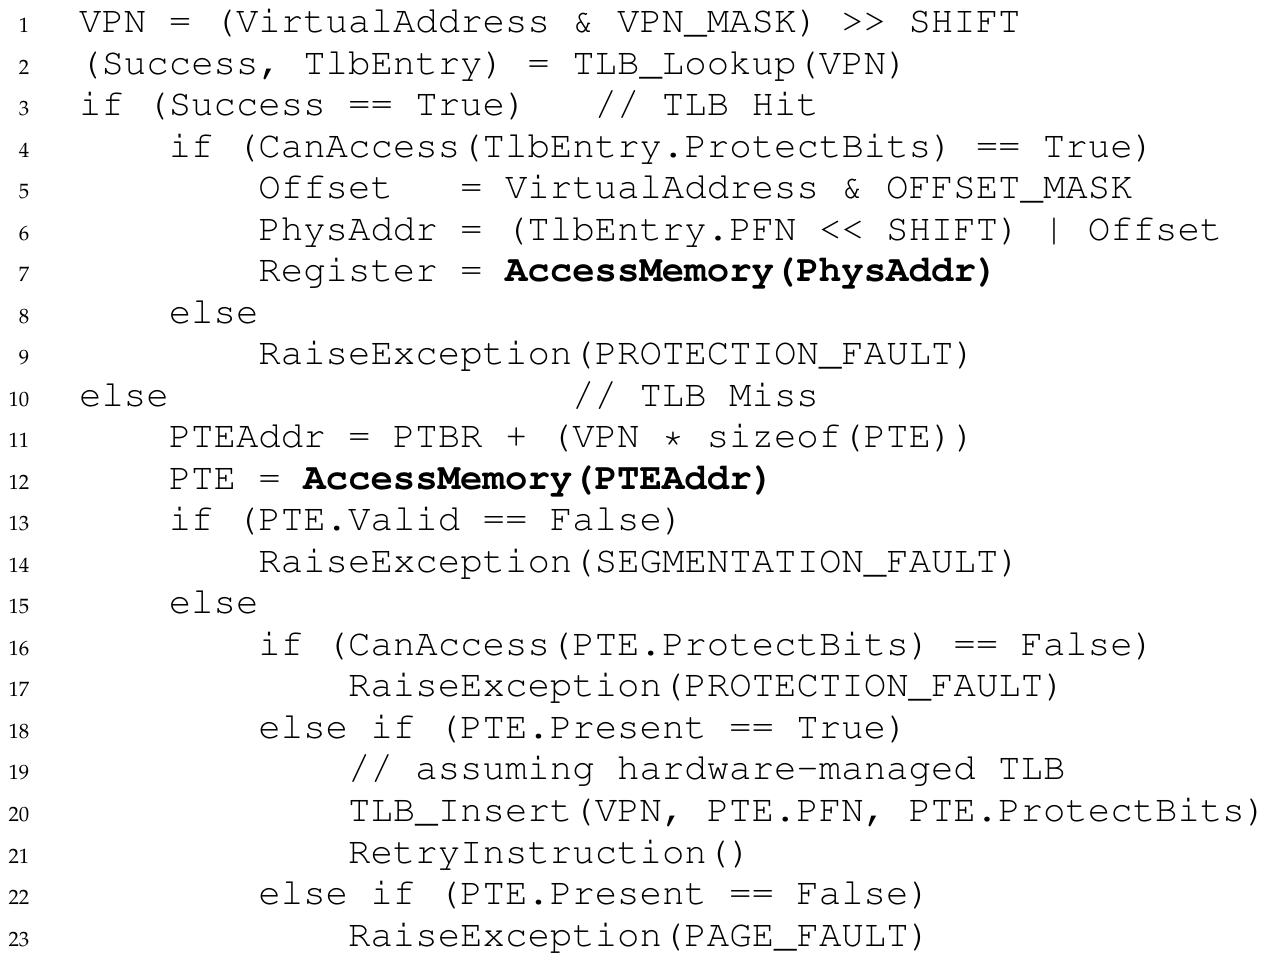
\includegraphics[width=1.0\linewidth]{figs/chapter-21/figure-21.2.png}
    \caption*{Source: chapter page 6.}
    \label{fig:figure-21.2}
\end{figure}

\end{columns}

\end{frame}

%------------------------------------------------
\begin{frame}{Page-Fault Control Flow: Software}

\begin{figure}
    \centering
    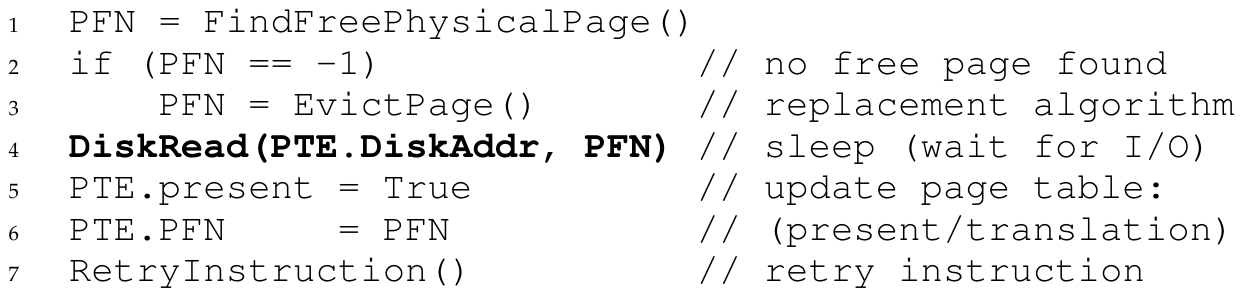
\includegraphics[width=0.85\linewidth]{figs/chapter-21/figure-21.3.png}
    \caption*{Source: chapter page 7.}
    \label{fig:figure-21.3}
\end{figure}

\begin{itemize}
    \item Find a free physical frame; if none, run the
          \textbf{replacement algorithm} to evict a page.
    \item Read the page from swap space (process sleeps during the I/O).
    \item Update the page table and retry: TLB miss, then TLB hit.
\end{itemize}

\end{frame}

%------------------------------------------------
\begin{frame}{When Replacements Really Occur}
\small

\begin{itemize}
    \item Waiting until memory is \textbf{entirely full} is unrealistic.
    \item OS keeps a small portion of memory free, using a
          \textbf{high watermark} (HW) and a \textbf{low watermark} (LW):
    \begin{itemize}
        \item fewer than LW free pages $\rightarrow$ a background thread
              evicts pages until HW pages are free;
        \item the thread is the \textbf{swap daemon} or
              \textbf{page daemon}.
    \end{itemize}
    \item Many replacements at once enable \textbf{clustering}: writing a group
          of pages to swap at once reduces disk seek and rotational overheads.
    \item The fault handler just checks for free pages and, if needed,
          wakes the background thread and waits.
\end{itemize}

\begin{block}{Tip: Do Work in the Background}
Background work increases efficiency, allows grouping of operations,
improves latency, may reduce work, and uses idle time.
\end{block}

\end{frame}

%------------------------------------------------
\begin{frame}{Summary}

\begin{itemize}
    \item Accessing \textbf{more memory than is physically present}.
    \item Page tables gain a \textbf{present bit}; when a page is not present,
          the \textbf{page-fault handler} brings it from disk, possibly
          replacing other pages first.
    \item All of this happens \textbf{transparently} to the process: it sees
          its own private, contiguous virtual memory.
    \item Common case is fast, but in the worst case a single instruction
          can take \textbf{many milliseconds}.
\end{itemize}

\end{frame}

%------------------------------------------------
\begin{frame}{Homework (Measurement)}

\begin{itemize}
    \item Tools: \texttt{vmstat} and the program \texttt{mem.c}.
    \item Run \texttt{vmstat 1} and \texttt{./mem 1}: how do the CPU usage
          statistics change? And with several instances?
    \item Watch \texttt{swpd} and \texttt{free} while running
          \texttt{./mem 1024} and after killing it.
    \item Use large sizes (check \texttt{/proc/meminfo}) and watch the swap
          columns \texttt{si}/\texttt{so}. How do the loops compare?
    \item Compare loop time and bandwidth when everything fits in memory
          versus constant swapping; check swap limits with \texttt{swapon -s}.
\end{itemize}

\end{frame}
